
A modo de introducción, comenzamos esta sección mostrando los datos demográficos obtenidos. Más adelante, continuamos con un análisis más exhaustivo de inteligibilidad y por separado se realizará otro análisis respecto a la nacionalidad atribuida a las oraciones. Por último para evaluar la hipótesis original, compondremos estos dos ejes para dilucidar el grado de validez de los resultados.

\section{Datos demográficos}

Se encuestaron $109$ participantes de los cuales se obtuvieron $352$ resultados. Del total de participantes, $49$ pertenecían al rango comprendido entre $18$ y $25$ años, $43$ estaban en el rango $26$-$35$. $17$ de los participantes eran mayores a $35$ años (fig. \ref{genero}).

\begin{figure}
\centering
\begin{subfigure}{.5\textwidth}
  \centering
	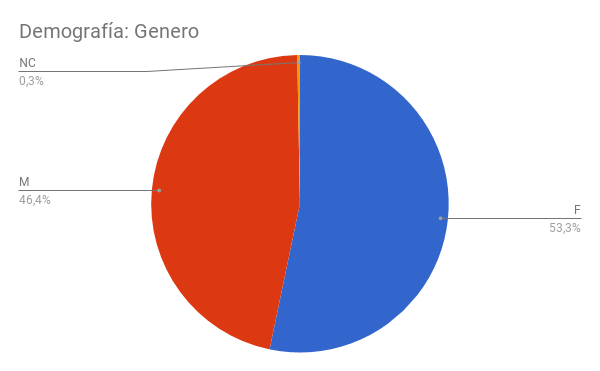
\includegraphics[width=1\linewidth]{datosDemograficos/genero.png}
  \caption{Género}
  \label{genero}
\end{subfigure}%
\begin{subfigure}{.5\textwidth}
  \centering
	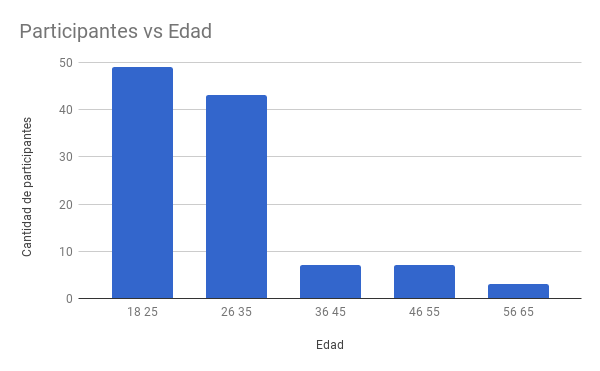
\includegraphics[width=1\linewidth]{datosDemograficos/edad.png}
  \caption{Edad}
  \label{fig:sub2}
\end{subfigure}
\caption{Datos demográficos de los participantes}
\label{edad}
\end{figure}

Con respecto al genero de los participantes, $187$ respuestas fueron brindadas por participantes del genero femenino mientras que $163$ respuestas fueron brindadas por participante del genero masculino (fig. \ref{edad}).

Con respecto de la región en que cada participante pasó su infancia puede verse una predominancia de personas del Gran Buenos Aires con $45\%$, seguido por un $30\%$ que pasaron su infancia en la Capital Federal. Menos del $25\%$ pertenece al resto de las provincias Argentinas. Además, $10$ personas contestaron que se criaron fuera del país (fig. \ref{distTerritorial}).

\begin{figure}
\begin{center}
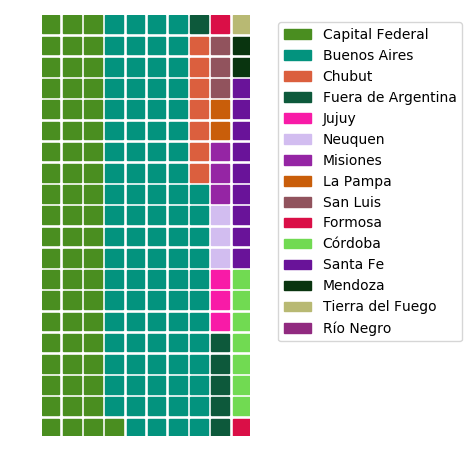
\includegraphics[scale=0.8]{datosDemograficos/infancia.png}
\end{center}
\caption{Distribución Territorial}
\label{distTerritorial}
\end{figure}

\section{Inteligibilidad}\label{SeccionInteligibilidad}

A continuación intentaremos medir la inteligibilidad de cada una de las oraciones en base a las respuestas obtenidas por los participantes. Para ello tomaremos la oración transcripta por los participantes y mediremos cuán lejos o cerca está de la oración original. 

Para esto utilizaremos la distancia de Levenshtein, que consiste en calcular la menor cantidad posible de inserciones, remociones o reemplazos de caracteres que son requeridos para transformar la oración transcripta por un participante en la oración objetivo. Así por ejemplo, para transformar \textit{cosa} en \textit{cal} se requieren $3$ transformaciones: reemplazar \textit{o} por \textit{a} final, reemplazar \textit{s} por \textit{l} y remover la \textit{a}. Por lo tanto, la distancia de Levenshtein entre estas dos palabras es de $3$. Además, se considerará un reemplazo cualquier acento, por lo que \textit{á} y \textit{a} tendrán distancia $1$ pero no así el reemplazo de mayúsculas y minúsculas, por lo que \textit{a} y \textit{A} tendrán distancia $0$.

En la figura \ref{resultadosGenerales} presentamos los resultados generales obtenidos sin ningún tipo de modificación a las transcripciones ingresadas por los sujetos. En el eje $x$ presentamos los grados de interpolación de inglés, yendo desde $30\%$ hasta $70\%$, mientras que en el eje $y$ presentamos la distancia de Levenshtein entre la oración objetivo y aquella transcripta por por cada participante. Cada uno de los boxplots describe la distancia mínima obtenida y la distancia máxima (los bigotes), como así también el primer y tercer cuartil (el piso y el techo de la caja) y la distancia media (linea interior que atraviesa la caja). Adicionalmente podemos observar con círculos vacíos los outliers de la muestra.


\begin{figure}
\begin{center}$
\begin{array}{lll}
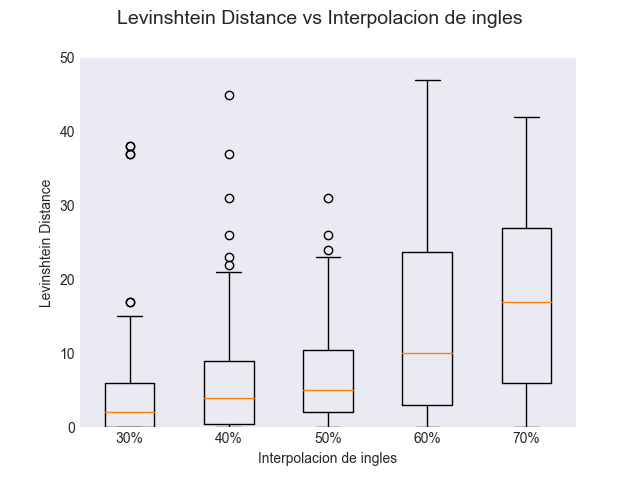
\includegraphics[width=.7\textwidth]{imagenes/plots_raw/general.png}
\end{array}$
\end{center}
\caption{Distancia de Levenshtein para distintos grados de interpolación}
\label{resultadosGenerales}
\end{figure}

Como puede observarse hasta el $50\%$ de interpolación de inglés, la distancia entre el primer y tercer cuartil es menor a $10$ caracteres, siendo la media de $5$. Pasados el $60\%$ de inglés, se observa un aumento brusco en la distancia intercuartiles, la distancia entre el primer y tercer cuartil pasa a ser cercana a $20$ caracteres, y la media $10$ caracteres en el caso de $60\%$ inglés y $15$ en el caso del $70\%$. En las próximas secciones intentaremos encontrar una explicación intuitiva a estos números.

\section{Problemas en las transcripciones y normalización}

Analizando detenidamente las transcripciones obtenidas pudimos observar algunas fallas sistemáticas que podrían generar ruido en el análisis. Por ejemplo algunos de los participantes escribieron de manera diferente las secciones de la oración que no comprendieron. Por citar algunos ejemplos, muchos de ellos escribieron: ``...'' o simplemente omitieron la palabra, mientras que una minoría escribió cosas como ``***'', ``???'', ``\textit{blablabla}''. En los casos donde el participante no comprendió ningún segmento de la oración, es común observar expresiones como ``\textit{no entendí nada}'', ``\textit{nada}'', etc.

Por otra parte es común la utilización innecesaria de signos de puntuación. Estos varían desde puntos finales para expresar el final de la oración hasta expresiones de confusión tales como ``(?)''. En un caso extremo, un participante transcribió \textit{``tu estrecho posavasos'', grito la fechoría}, cuando la oración original solo decía \textit{tu estrecho portavasos gritó la fechoría}.
También pueden verse omisiones de acentos y faltas ortográficas en palabras que no presentan ambigüedades, como por ejemplo: ``grunion'' en vez de ``gruñón''.

Todas estas expresiones y modismos tienen como consecuencia directa que la distancia de Levenshtein se vea afectada. Por ejemplo, un participante que haya escrito ``\textit{no entendí nada}'' como respuesta devolverá una distancia distinta de aquel que simplemente dejó el campo vacío, cuando en realidad expresan el mismo grado de compresión del texto.

Con el objetivo de reducir esta variabilidad en la muestra, se decidió realizar una limpieza de los datos. Buscamos uniformizar los datos para un mejor análisis, intentando mantener siempre el espíritu de la respuesta dada por el participante. De esta manera consideramos que si un participante escribió ``...'' en medio de una oración, lo que quiso decir es que no comprendió parte de la misma. Hubiera sido igual que en su lugar hubiese escrito la cadena vacía ``'', por ejemplo.

De esta manera consideramos que los siguientes cambios no presentan alteraciones graves en las respuestas de los participantes:

\begin{itemize}
	\item Corrección de ``ni'' por ``ñ'' en la palabra \textit{grunion}.
	\item Remoción de todos los signos de puntuación: comas, puntos, ``(?)''
	\item Reemplazo de oraciones como \textit{blabla}, \textit{no entendí} o cualquier otra expresión que indique ininteligibilidad de una palabra u oración por la cadena vacía ``''.
	\item Corrección de acentos en palabras no ambiguas: \textit{botón}, \textit{prefirió}, \textit{recorrió}, \textit{chupetín}, \textit{riñón}, \textit{gruñón}.
\end{itemize}

Aquellas palabras que presentan alguna ambivalencia, como \textit{concluyo}, no fueron modificadas ya que tanto \textit{concluyó/concluyo} son válidas. El participante podría haber interpretado la palabra con cualquiera de las dos connotaciones cambiando el significado de la interpretación y su distancia de Levenshtein.

Esperamos que esta limpieza nos ayude a disminuir el error de los resultados y también, nos permitirá interpretar de manera más intuitiva el significado de la distancia de Levenshtein en cada caso.

\clearpage

\section{Datos normalizados} \label{datosNormalizados}

De manera similar que en el apartado anterior, en la figura \ref{generalNormalizado} presentamos los resultados esta vez con los datos normalizados.

\begin{figure}
\begin{center}$
\begin{array}{lll}
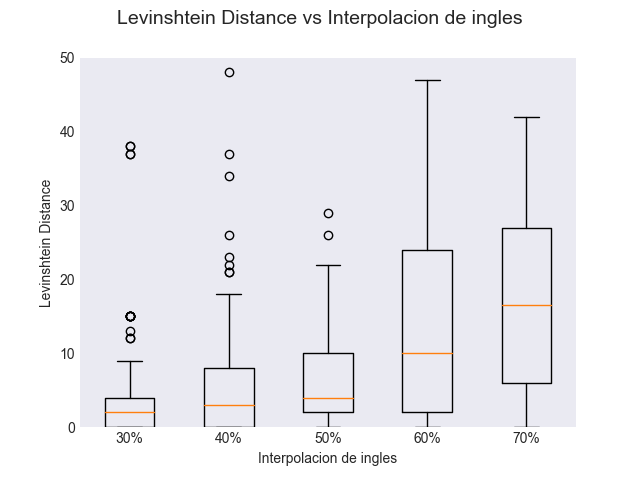
\includegraphics[width=.7\textwidth]{imagenes/plots_normalized/general.png}
\end{array}$
\end{center}
\caption{Distancia de Levenshtein para distintos grados de interpolación con datos normalizados}
\label{generalNormalizado}
\end{figure}

En esta figura podemos observar que para una interpolación de inglés de $30\%$, $96$ de los $106$ participantes obtuvieron una distancia menor a los $10$ caracteres en la transcripción del texto, mientras que los $10$ restantes una distancia mayor a los $10$ caracteres. Podemos ver además que la distancia entre el primer y tercer cuartil es menor a $5$ caracteres con una media cercana a $2$ 

Para la mezcla con $40\%$ de interpolación de inglés, de un total de $67$ participantes, $57$ anotaron una distancia de Levenshtein menor a diez caracteres, $7$ una distancia entre $10$ y $30$ caracteres y $3$ una distancia mayor a $30$. La distancia intercuartil es de aproximadamente diez caracteres, con una media muy similar a la mezcla $30\%$ inglés.

Para la interpolación $50\%$ de inglés, de un total de $75$ participantes, $57$ lograron transcribir el audio con una distancia menor a $10$ caracteres, mientras que $14$ anotaron una distancia entre $10$ y $20$ caracteres y $4$ una distancia mayor a $20$. De manera similar que para $40\%$ la distancia intercuartil es de aproximadamente diez caracteres y la media es de $3$ caracteres.

Ademas, con esta estandarización de los datos, trataremos de darles un peso intuitivo que nos permitan sistematizar el análisis.

Por ejemplo, tomando la oración $8$ de las frases utilizadas en la experimentación: 

\begin{itemize}
	\item ``Las acongojadas cotorras sonrieron a mi círculo''
\end{itemize}

Podemos observar las siguientes transcripciones extraídas de los resultados:

\begin{itemize}
	\item Distancia 0: ``Las acongojadas cotorras sonrieron a mi círculo''
	\item Distancia 10: ``Las acontojadas culturas sonrieron en semicírculo''
	\item Distancia 20: ``Plaza sombreada con sombrero sonrieron en mi círculo''
	\item Distancia 30: ``sonrieron en mi círculo''
	\item Distancia 40: ``círculo''
	\item Distancia 48: ``''
\end{itemize}

Para todas las interpolaciones enunciadas previamente, los errores mas comunes varían desde falta de acentos en palabras como ``concluyó'' hasta faltas de inteligibilidad en palabras con cierta complejidad fonética como ``aguileña'' o ``gruñón''.

Como caso particular la oración $3$: ``este enjoyado juez comprará nuestro corchete'' podemos observar que la mayoría de los participantes cometieron errores al transcribir la palabra ``juez'', que confundieron de manera sistemática con palabras sonoramente similares como ``fue'', ``enjoyado'', que transcribieron como ``enfollado'' o ``enrollado'', y la conjugación del verbo ``comprar'' que transcribieron como ``comprando'' o ``comprar''.

Buscando una explicación a estos errores y revisando el mapeo de fonemas que realizamos previamente, descubrimos que el mapeo de /hh/ a /g/ era erróneo. Esto produjo que palabras como ``gato'' sonaran mas como ``jato'' (/hh/ /a/ /t/ /o/). Adicionalmente descubrimos que ningún fono del inglés estaba siendo mapeado al fono /x/. Esto produjo que cuando el sintetizador interpola entre entre el fono del castellano y el fono inexistente del inglés (que hts toma como ruido blanco), el resultado fuera una mezcla entre ruido y /x/. Al ser la /x/ ruido blanco (consonante fricativa), no pudimos reconocer el error en las instancias preliminares de evaluación. Esto explicaría porque algunos participantes tuvieron problemas transcribiendo la palabra ``juez''.

Para los grados de interpolación $60\%$ y $70\%$ inglés, podemos observar un aumento notable de la variabilidad en las respuestas. Para el primero, de las $70$ respuestas obtenidas, $40$ participantes lograron transcribir el audio con una distancia menor a diez caracteres, $6$ obtuvieron anotaron una distancia entre $10$ y $20$ caracteres, y $24$ transcribieron el audio con distancia mayor a veinte caracteres. La distancia entre el primer y tercer cuartil pasa a ser de $20$ caracteres con una media igual a $10$.

Para $70\%$ inglés, la diferencia es todavía mas marcada, de los $68$ resultados obtenidos, $28$ lograron transcribir el audio con un buen grado de inteligibilidad, $8$ con un grado medio y $32$ con un grado bajo o nulo de inteligibilidad. La distancia intercuartil se mantiene similar a la de mezcla $60\%$ inglés, aproximadamente $20$ caracteres pero vemos un salto en la media que ahora es de $20$ caracteres.

Consideramos que este salto en la distancia intercuartil puede deberse a dos motivos: El primero es que existen características particulares de los participantes y sus capacidades para discernir palabras, incluso cuando presentan defectos en la pronunciación del hablante. En particular, la oración $4$ (ver figura \ref{oracionCuatro}) muestra cómo para el $70\%$ de inglés - $30\%$ de español en la interpolación, $2$ participantes de los $9$ que realizaron la transcripción, obtuvieron distancias $2$ y $6$ en sus transcripciones.

\begin{figure}
\begin{center}$
\begin{array}{lll}
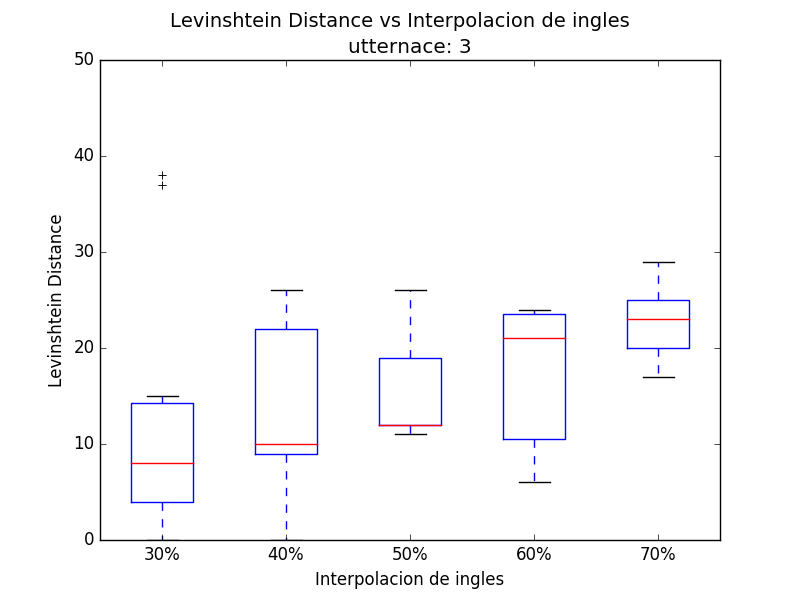
\includegraphics[width=.5\textwidth]{imagenes/plots_normalized/3.png}
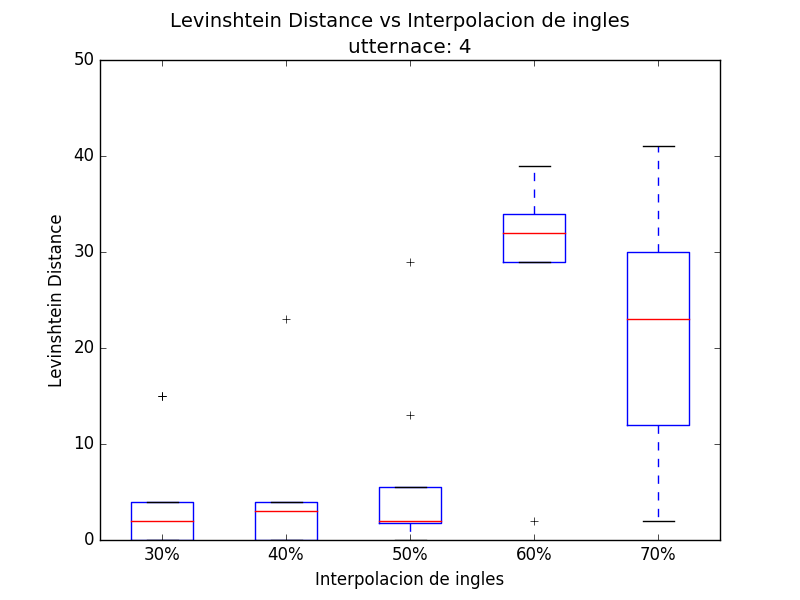
\includegraphics[width=.5\textwidth]{imagenes/plots_normalized/4.png}
\end{array}$
\end{center}
\caption{Oración 4 Normalizada}
\label{oracionCuatro}
\end{figure}

El segundo motivo puede deberse a que existen características particulares de las oraciones o del modelo utilizado para generar la voz que afectan la comprensión del audio: la oración $10$ ``El nudillo Argentino perdió su vaso'' con $70\%$ de interpolación de inglés - $30\%$ de castellano, en la cual $6$ de los $8$ participantes obtuvieron una buena transcripción del audio con distancia menor a $15$ \footnote{Incluso teniendo en cuenta que esta oración se ve afectada por el mapeo incorrecto de la /g/ como fue discutido previamente}, y la oración $8$ ``Las acongojadas cotorras sonrieron a mi círculo'', donde, para ese mismo grado de interpolación, todos los participantes transcribieron el audio con distancia de Levenshtein mayor a $20$, parecen demostrar esto. O bien la dificultad de las oraciones es variable o, lo que es todavía mas probable, llegado cierto punto en la interpolación, algunos fonemas empiezan a ``romperse'' o se alejan demasiado del fonema castellano correcto y terminan por disminuir la claridad de la voz.

\begin{figure}
\begin{center}$
\begin{array}{lll}
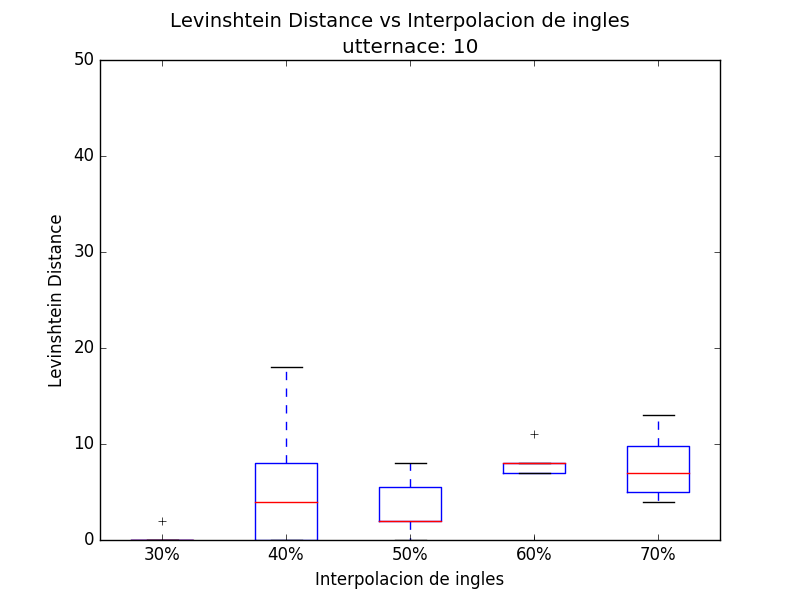
\includegraphics[width=.5\textwidth]{imagenes/plots_normalized/10.png}&
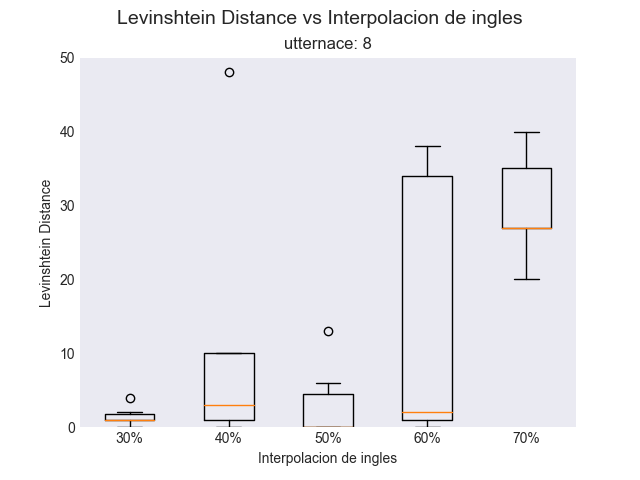
\includegraphics[width=.5\textwidth]{imagenes/plots_normalized/8.png}
\end{array}$
\end{center}
\caption{Oración 10 y 8 Normalizados}
\label{pics:blablabla}
\end{figure}

En conclusión, en esta sección pudimos demostrar que fue posible generar una voz con una distancia menor a $10$ caracteres hasta un $50\%$ de inglés y $50\%$ de castellano. Pasado el $50\%$ de inglés, la variabilidad de las respuestas se vuelve mucho mas grande pudiendo haber participantes que anotan una buena distancia de Levenshtein ($10$ caracteres o menos) hasta algunos que no logran comprender ni siquiera segmentos aislados del mismo (mas de $30$ caracteres).

% \begin{figure}
% \begin{center}$
% \begin{array}{lll}
% 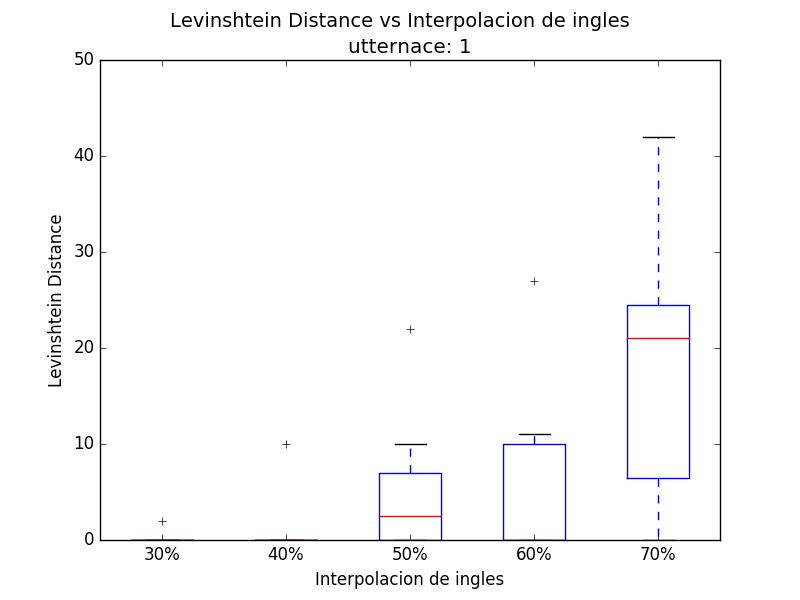
\includegraphics[width=.5\textwidth]{imagenes/plots_normalized/1.png}&
% 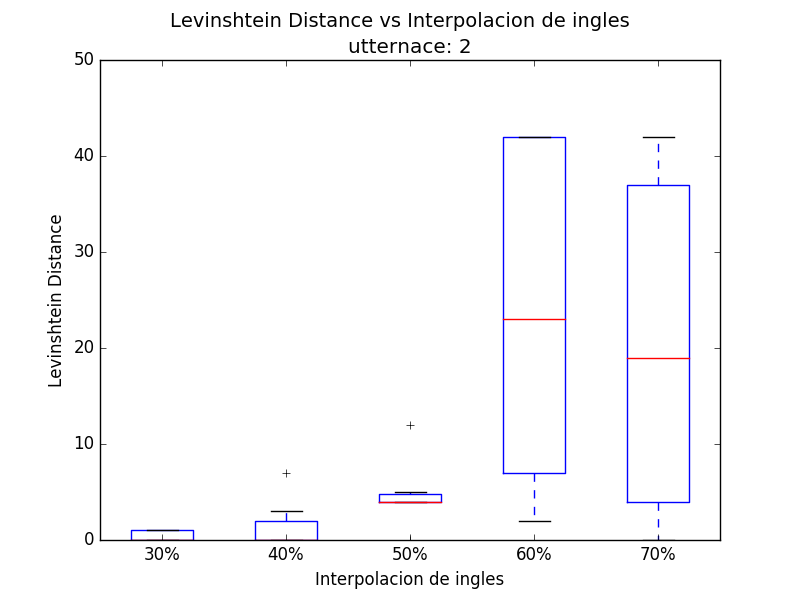
\includegraphics[width=.5\textwidth]{imagenes/plots_normalized/2.png}
% \end{array}$
% \end{center}
% \caption{Utternace 1 y 2 Normalizados}
% \label{pics:blablabla}
% \end{figure}

% \begin{figure}
% \begin{center}$
% \begin{array}{lll}
% 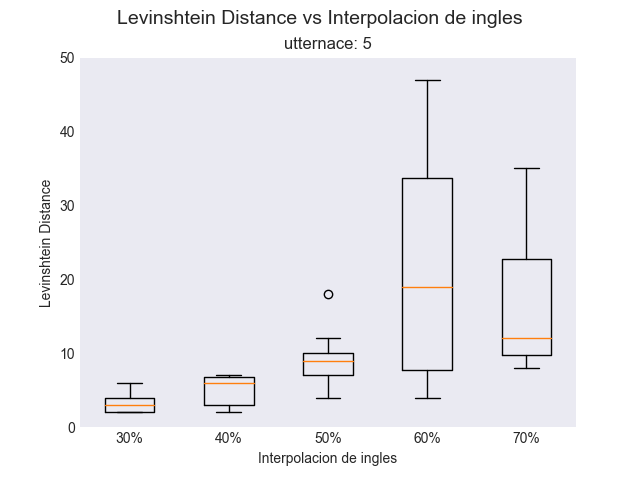
\includegraphics[width=.5\textwidth]{imagenes/plots_normalized/5.png}&
% 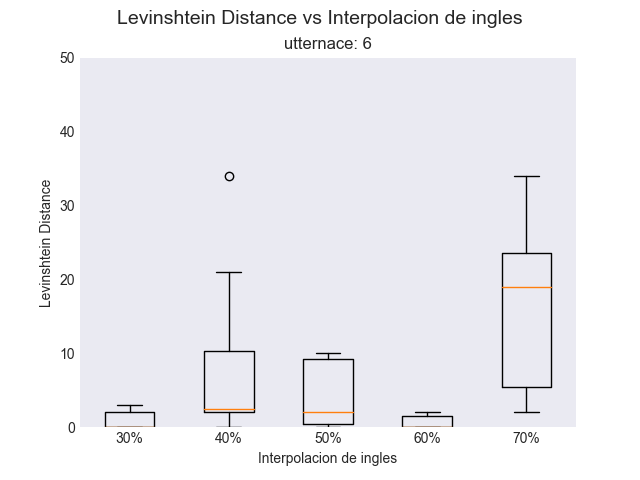
\includegraphics[width=.5\textwidth]{imagenes/plots_normalized/6.png}
% \end{array}$
% \end{center}
% \caption{Utternace 5 y 6 Normalizados}
% \label{pics:blablabla}
% \end{figure}

% \begin{figure}
% \begin{center}$
% \begin{array}{lll}
% 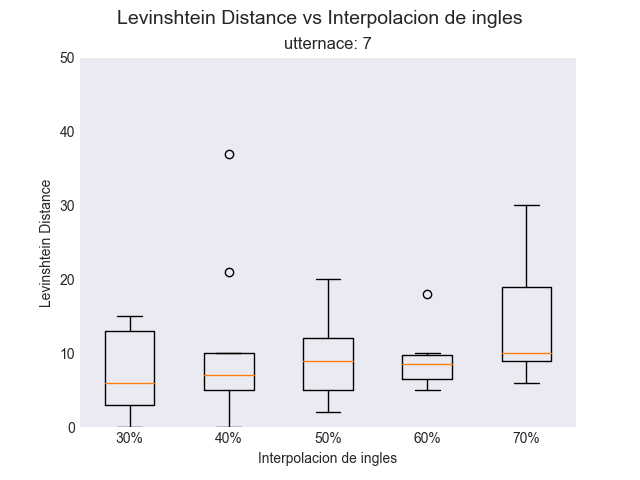
\includegraphics[width=.5\textwidth]{imagenes/plots_normalized/7.png}&
% 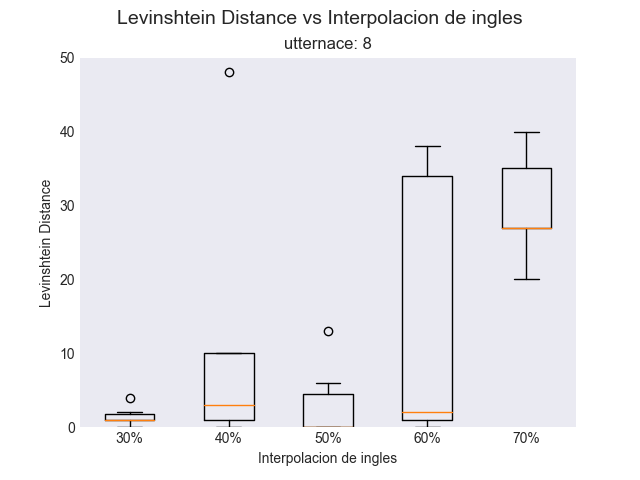
\includegraphics[width=.5\textwidth]{imagenes/plots_normalized/8.png}
% \end{array}$
% \end{center}
% \caption{Utternace 7 y 8 Normalizados}
% \label{pics:blablabla}
% \end{figure}


%Agregar:
% python LevenshteinFor.py 0
% Alta int: 96
% Media int: 10
% Baja int: 0
% nula: 4
% python LevenshteinFor.py 1
% Alta int: 57
% Media int: 2
% Baja int: 5
% nula: 3
% porque nula? ver esto: parecen ser outliers
% python LevenshteinFor.py 2
% Alta int: 57
% Media int: 14
% Baja int: 4
% nula: 0
% python LevenshteinFor.py 3
% Alta int: 40
% Media int: 6
% Baja int: 11
% nula: 13
% python LevenshteinFor.py 4
% Alta int: 28
% Media int: 8
% Baja int: 20
% nula: 12


\clearpage
\section{Análisis del Origen Percibido}

En esta sección analizaremos los resultados de los orígenes o nacionalidades que los participantes de la encuesta atribuyeron a la voz.

Dado que en esta instancia se le permitió a los participantes ingresar texto libre las respuestas resultaron bastante heterogéneas. Los participantes interpretaron la consigna de distintas maneras, pudiendo encontrarse respuestas que no pueden ser atribuidas a una nacionalidad. Como ejemplo de algunas respuestas pueden encontrarse cosas como: ``Latino'', ``Anglo'', ``Robot'', ``España (sur)''.

Consideramos que las respuestas de la índole ``robot'', ``es una voz artificial'',no aportan información para esta investigación.

Por esta razón, en esta instancia decidimos agrupar las respuestas en cuatro conjuntos:

\begin{itemize}
	\item Hispanoparlate: ``Latino'', ``Argentino'', ``Español'', ``Uruguayo'', ``Centroamericano'', ``Boliviano'', `` Mexicano'',``Colombiano''.
	\item Angloparlante: ``Estadounidense'', ``inglés'', ``Irlandés'', ``Canadiense'', ``Anglo''.
	\item No sabe/No contesta: ``Robot'', ``no se''.
	\item Otro: ``Ruso'', ``Brasiltiño'' (sic).
\end{itemize}

Con estas agrupaciones, en la figura \ref{analGeneral} presentamos las nacionalidades atribuidas a la voz generada para cada punto de la interpolación.

\begin{figure}
\begin{center}$
\begin{array}{lll}
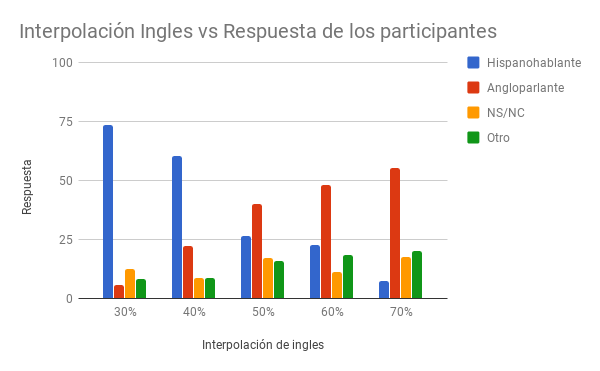
\includegraphics[width=.7\textwidth]{imagenes/nacionalidades/general.png}
\end{array}$
\end{center}
\caption{Análisis General}
\label{analGeneral}
\end{figure}

De estos resultados podemos observar que con $30\%$ de interpolación de inglés, los participantes coinciden ampliamente en que la voz puede atribuirse a una persona de habla nativa española.

En la figura pueden verse dos tendencias muy marcadas. La primera es que, a medida que aumenta el grado de interpolación de inglés, disminuye de manera lineal la cantidad de participantes que afirman que el hablante es Hispanohablante. Dicho de otra manera, los datos parecen sugerir que con cada salto en la interpolación inglés, la cantidad de participantes que afirma que la voz pertenece a un Hispanohablante, disminuye en aproximadamente $7$ puntos conceptuales. 

Una tendencia opuesta puede notarse en los participantes que afirman que la voz es de un hablante anglosajón. A medida que aumenta el grado de interpolación de inglés, el porcentaje de atribuciones de la voz a un hablante Anglosajón aumenta aproximadamente en un $7
\%$ cada vez.

Por otro lado, tanto para el conjunto ''Otro´´ como para ''NS/NC´´ podemos apreciar un leve aumento monotono entre los aumentos de interpolación de ingles.

%Con interpolación $50\%$ de inglés - $50\%$ de castellano y $60\%$ inglés - $40\%$ castellano, los resultados son similares: aproximadamente en la mitad de las oraciones, mas de la mitad de los participantes consideraron que la voz pertenecía a un anglosajón hablando castellano. Para estos grados de interpolación también podemos observar que en un $80\%$ de las oraciones al menos un $20\%$ de los participantes atribuyen la nacionalidad del hablante a extranjero de origen no anglosajón hablando castellano.

%Con $70\%$ de interpolación, en el $80\%$ de las oraciones se puede apreciar que al menos $50\%$ de los participantes dijo que el hablante era de origen anglosajón. Mas aún, en el $40\%$ de las oraciones el $75\%$ de los participantes coincidió que la voz era de angloparlante. También podemos ver que para este grado de interpolación en el $70\%$ de las oraciones ningún participante considera que la voz sea de habla hispana. En el $30\%$ restante, $25\%$ de los participantes o menos consideran que la voz pertenezca a un hispanohablante.

%grafico general mostrando como crece el grado de inglés?

%conclucion mas general: aunque en muchos casos los participantes atribuyeron a la voz como un extrangero no Anglosajón, tambien tener en cuenta que se esta intentando identificar la nacionalidad de un hablante con tan solo con una oración como referencia.

Observando las oraciones una por una, podemos algunas dicrepancias con los resultados generales. Por ejemplo, en la oración $9$(``Ese gruñón perro prometió a esos cuñados''), con un $40\%$ de interpolación de ingles,\cuantoEsParaGeneral el $60.00\%$ de los participantes considera que la voz pertenece a un hablante de habla anglosajona.

\begin{figure}
\begin{center}$
\begin{array}{lll}
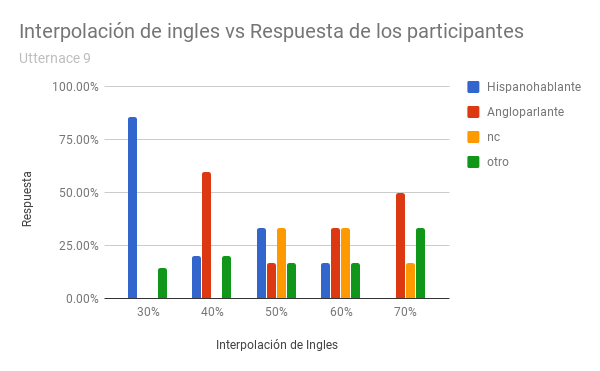
\includegraphics[width=.7\textwidth]{imagenes/nacionalidades/9.png}
\end{array}$
\end{center}
\caption{Oración 3 y 9}
\label{tresNueve}
\end{figure}

Esta gran disparidad en los resultados se puede atribuir a las características particulares de cada oración. En particular la oración $9$ contiene una /\textipa{r}/ (\textit{perro}) que resulta muy notoria al pronunciarse con una intensidad menor a la esperada (mas similar a una /\textipa{R}/ (\textit{pero})) y puede ser atribuida, entre otras causas, a un hablante Anglosajón con dificultades en la dicción de fonemas extranjeros.
%perro vibrante múltiple alveolar sonora

Bajo esta suposición observamos que las otras oraciones que presentan este fonema:

\begin{itemize}
\item Oración $1$: ``Mi montaña aguileña recorrió la esquina'' 
\item Oración $6$: ``Su profundo riñón apoyó a Julio''
\item Oración $7$: ``El frío churrasco oyó lo de Polonia''
\item Oración $8$: ``Las acongojadas cotorras sonrieron a mi círculo''
\end{itemize}

En la figura \ref{unoSeis} podemos observar que las oraciones $1$ y $7$ tambien tienen una marcada diferenciación respecto a los resultados generales. En particular estas dos oraciones no describen el comportamiento monotono observado previamente. 


\begin{figure}
\begin{center}$
\begin{array}{lll}
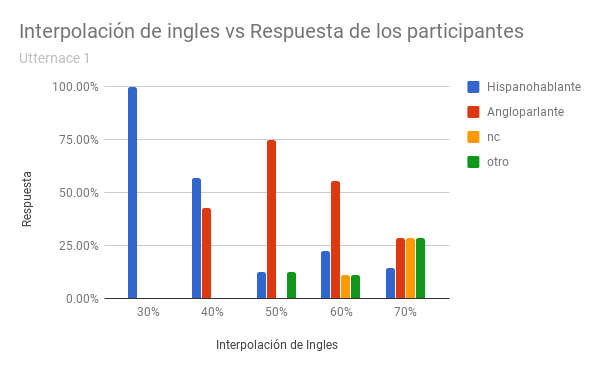
\includegraphics[width=.5\textwidth]{imagenes/nacionalidades/1.png}&
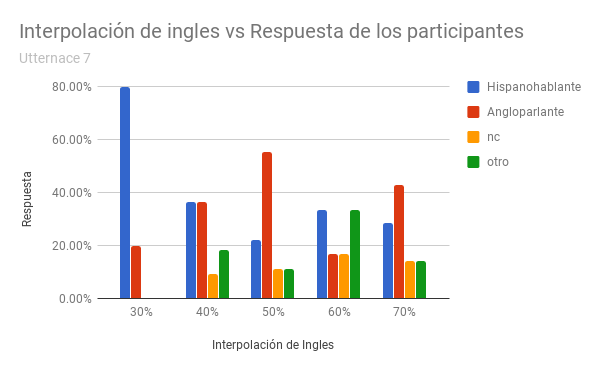
\includegraphics[width=.5\textwidth]{imagenes/nacionalidades/7.png}
\end{array}$
\end{center}
\caption{Oración 1 y 6}
\label{unoSeis}
\end{figure}

Por otro lado en la figura \ref{sieteOcho} plasmamos de manera grafica los datos obtenidos para la figura $6$ y $8$. En estos casos no pueden observarse diferencias que resulten notorias al compararlos contra los resultados generales.

\begin{figure}
\begin{center}$
\begin{array}{lll}
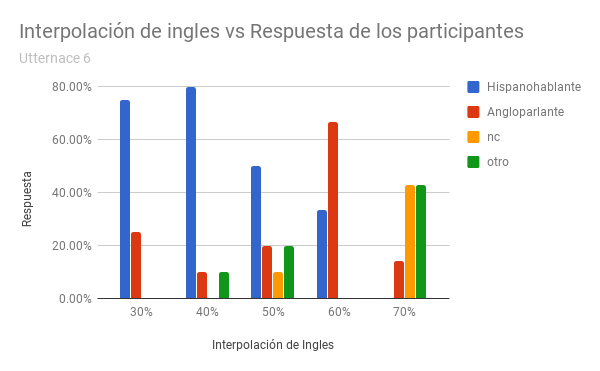
\includegraphics[width=.5\textwidth]{imagenes/nacionalidades/6.png}&
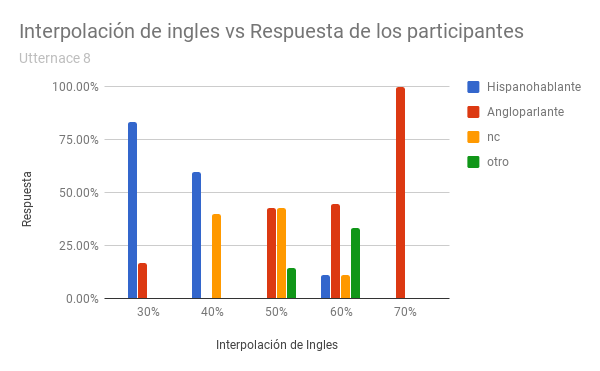
\includegraphics[width=.5\textwidth]{imagenes/nacionalidades/8.png}
\end{array}$
\end{center}
\caption{Oración 7 y 8}
\label{sieteOcho}
\end{figure}

Hasta ahora analizamos los dos ejes de nuestra hipótesis por separado (por un lado, inteligibilidad, por otro, nacionalidad atribuida a la voz). En el ultimo apartado de la investigación buscaremos sacar conclusiones al componer ambos ejes en un mismo análisis.

\section{Resultados Generales de la experimentación}

En la figura \ref{resultadosGeneralesNacVsPlot} presentamos los resultados comparando las distancias de Levenshtein con los porcentajes de participantes que determinaron que el hablante fuera Anglosajón. Al igual que en el apartado \ref{SeccionInteligibilidad}, en el eje $x$ presentamos los grados de interpolación de inglés, yendo desde $30\%$ hasta $70\%$. El eje $y$ del lado izquierdo representa la distancia de Levenshtein  entre la oración objetivo y aquella transcripta por por cada participante. Cada uno de los boxplots describe la distancia mínima obtenida y la distancia máxima (los bigotes), como así también el primer y tercer cuartil (el piso y el techo de la caja) y la distancia media (linea interior que atraviesa la caja). En el eje $y$ del lado derecho, presentamos el porcentaje de participantes que atribuyeron la voz a un hablante anglosajón indicadp mediante puntos verdes en el grafico. Adicionalmente podemos observar con círculos vacíos los outliers de la muestra.

\begin{figure}
\begin{center}$
\begin{array}{lll}
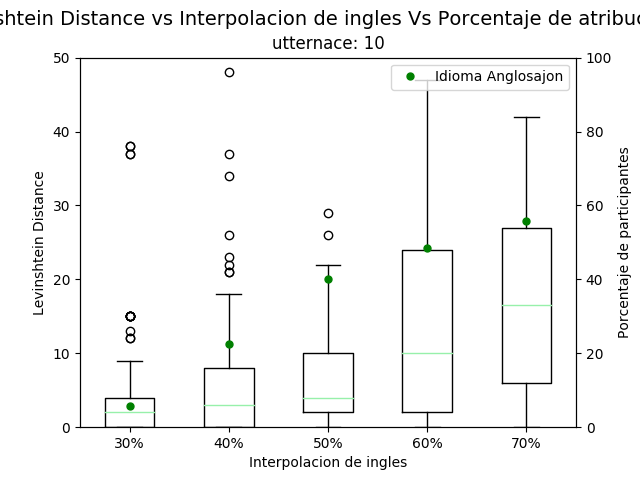
\includegraphics[width=.7\textwidth]{imagenes/nacVsPlot/general.png}
\end{array}$
\end{center}
\caption{Distancia de Levenshtein vs distintos grados de interpolación vs Porcentaje de participantes que consideran hablante anglosajón}
\label{resultadosGeneralesNacVsPlot}
\end{figure}

En esta figura podemos apreciar que para cada aumento en el grado de interpolación de inglés, tanto el porcentaje de participantes que considera la voz como un hablante anglosajón como la media de la distancia de Levenshtein crecen de manera monotona. Comenzando con un $5\%$ de participantes afirmando que la voz anglosajona y una media de la distancia de Levenshtein de $3$ para una interpolación de $30\%$ inglés, y llegando hasta $55\%$ de participantes afirmando que la voz pertenecía a un hablante anglosajón y una distancia de Levenshtein media de aproximadamente $18$ caracteres para la interpolación de $70\%$ inglés.

En base a estos resultados podemos afirmar que la hipótesis original tiene cierto grado de validez experimental: la interpolación de HMMs descripta en esta tesis es un método valido para generar voces que pueden ser identificadas con un nativo anglosajón hablando castellano. Sin embargo esto viene con un costo asociado: la claridad de las oraciones disminuirá a medida que se aumenta el grado de interpolación del modelo de inglés.

\unificarGradoInglesGradoCastellanoAGradoIngles
\IntroducirEstaNomenclatura